\chapter{Split Ring Resonator}


In the work done by Xu et al \cite{Xu2021}, the plasma discharge was generated using a CCP jet, specifically a design by the European Cooperation in Science and Technology (COST) \cite{Gorbanev2019}. The COST plasma jet was originally developed for medical and biomedical applications, as such were developed to operate at the approved ISM frequency of 13.56 MHz. However, RF plasma sources are flawed in the sense that they have a limited plasma density, which could theoretically limit the rate of splitting of CO$_2$ molecules.

To mitigate this, this project attempts to emulate the process of CO$_2$ splitting using a micowave plasma, specifically a microstrip-based source called the \textit{split ring resonator} (SRR). Using such a device will have three benefits. First, the power efficiency of the micowave plasmas would allow for discharges to occur on the order of milliwatts (mWs) rather than watts (W). The device would also be much smaller and cheaper to manufacture. Finally, as mentioned in section \ref{subsec:microwave_discharge}, operating at a higher frequency should increase the plasma density.

An illustration of an SSR can be seen in figure \ref{fig:SRR}. The design of a SRR is quite simple, consisting of a conducting ring, usually made of copper, laid on top of a dielectric substrate. The bottom of the dielectric consist of a ground plane that covers the entirety of the surface. This has the added benefit of dispersing the heat generated from the SRR. As seen in figure \ref{fig:SRR}, there is a small gap made on the top surface that breaks the copper ring, which is where the plasma discharge occurs. 


\begin{figure}[h!]
	\centering
	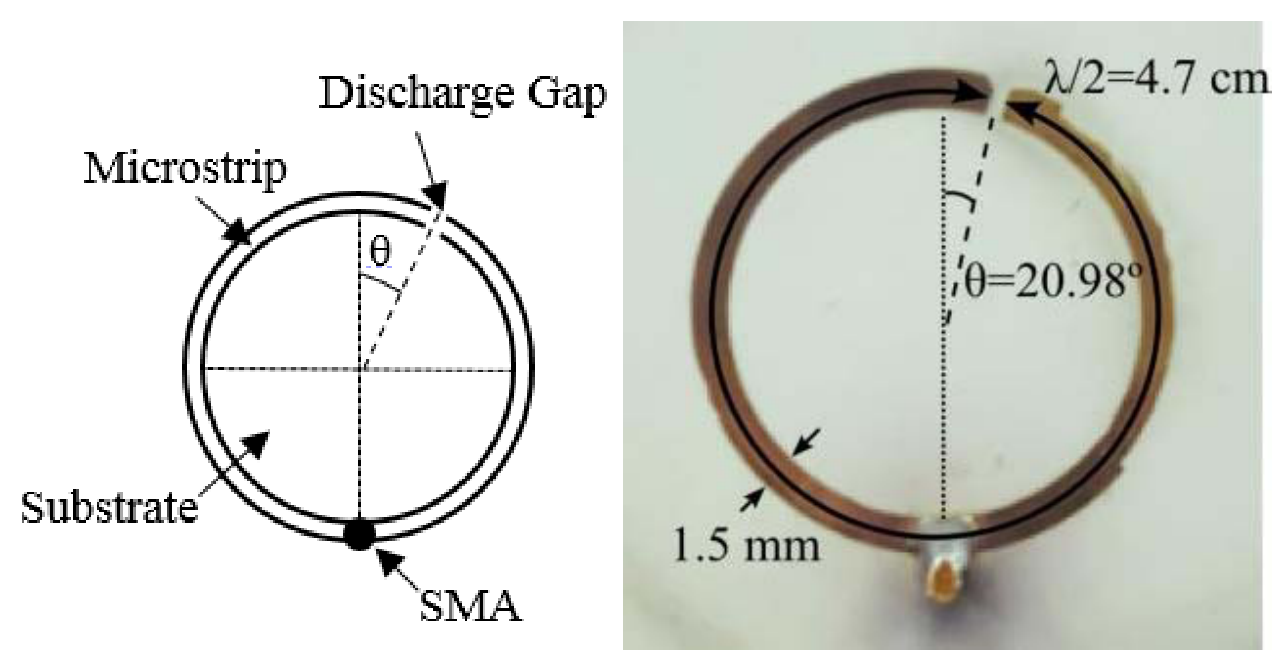
\includegraphics[width=0.7\linewidth]{chapter_4/figures/split_ring_resonator.png}
	\caption{Schematic (left) and photo (right) of SRR \cite{Dextre2017}.}
	\label{fig:SRR}
\end{figure}

\section{Overview}


In order to achieve a discharge, a high frequency (microwave) voltage is applied to the SRR via the SMA connector. The exact frequency to be used is governed by two factors: the mean circumference (which is measured from the middle) of the top conducting ring and the dielectric constant of the substrate used. The mean circumference is specifically designed to be half the wavelength corresponding to the desired frequency. The dielectric constant is required to determine the speed of light in the dielectric medium used. Thus, an equation for the frequency used for a given SRR is \cite{Dextre2017}:

\begin{equation}
     f = \frac{c}{\lambda\sqrt{\varepsilon_r}}
     \label{eq:resonant_frequency}
\end{equation}

The reason why the mean circumference is designed to be half the desired wavelength is for power efficiency. Due to this design, the ends of the SRR (i.e. where the gap is) will be $180^\circ$ out of phase from each other. Because of this, when one end of the SRR is at the peak of the AC cycle, the other will be at a trough; thus the potential difference between the two ends has been doubled. This geometric trick allows for the doubling of the strength of the electric field at a constant power. 
% TODO (Future): Explain this better

Astute readers may notice another peculiarity with the SRR seen in figure \ref{fig:SRR}, in that it is not symmetrical. Instead, the discharge gap appears to be offset towards one side of the device. This is deliberate as the offset gap allows for the impedance matching of the SRR to the impedance of the power supply used, thus maximising the power transfer. This offset angle is measured from the very centre of the ring, and is determined using the expression \cite{Iza2005}:

\begin{equation}
	\theta = arccos(1 - \frac{Z_{in} \pi}{Z_0 Q})
	\label{eq:offset_angle}
\end{equation}


where $Z_{in}$ is the input impedance of the power supply, $Q$ is the quality factor, and $Z_0$ is the characteristic impedance of the SRR. Typically, the input impedance of many power supplies is 50 $\Omega$. The characteristic impedance is governed by four factors: the width of the top copper trace, the thickness of the copper pour, the thickness of the dielectric substrate, and the dielectric constant of the substrate. Wheeler derived an analytical solution, see equations \ref{eq:wheeler_microstrip}-\ref{eq:wheeler_effective_w}, that approximates the characteristic impedance with an error of less than 1\% \cite{wheeler_1977}. As for the quality factor, this parameter is given on the data sheet of the substrate used.

\begin{equation}
    Z_0 = \frac{42.4}{\sqrt{1+\varepsilon_r}}\left[ 1 + \frac{4h}{w'}(X_1 + X_2)\right]
    \label{eq:wheeler_microstrip}
\end{equation}
\begin{equation}
    X_1 = \frac{4h}{w'}\left(\frac{14\varepsilon_r + 8}{11\varepsilon_r}\right)
\end{equation}
\begin{equation}
    X_2 = \sqrt{\left(\frac{4h}{w'}\right)^2 \left(\frac{14\varepsilon_r + 8}{11\varepsilon_r}\right)^2 + \pi^2\frac{1+\frac{1}{\varepsilon_r}}{2}}\
\end{equation}
\begin{equation}
    w' = w + \frac{t}{\pi}ln\left[\frac{4e}{\sqrt{(\frac{t}{h})^2 + (\frac{t}{w\pi + 1.1\pi})^2}}\right]\frac{\varepsilon_r + 1}{2\varepsilon_r}
    \label{eq:wheeler_effective_w}
\end{equation}

where $w$ is the width of the top copper trace, $t$ is the thickness of the copper pour (typically specified by the PCB manufacturer), and $h$ is the height of the dielectric substrate. 

\section{Production}

The SRR device used in this project introduces a slight modification to the design of the traditional SRR. In order to create a small jet of plasma, through holes are needed at the region of the gap of the SRR. This would allow the gases to react with the plasma, then pass through the hole.

However, to determine if this small change had any significant effects on the behaviour of the SRR, simulations were run to better understand the discharge dynamics. Specifically, \textit{Particle-in-cell} (PIC) simulations were used; and the software used is called \textit{XOOPIC} \cite{Verboncoeur1995}. Further information on PIC simulations and XOOPIC can be found in the appendices. 

\subsection{Simulations}

Multiple different simulations were run to understand the characteristics of the plasma, however they could be broadly broken down into three groups. For all these simulations, a cross sectional plane of the discharge gap of the SRR was modelled. The reasoning for this was that the plasma formed would typically be constrained around the gap \cite{iza2003}. Though the ring of the SRR is a circle, the discharge gap is small relative to the overall device, hence can be approximated to be a rectangle. For all the following simulations, the parameters can be found in table \ref{tb:basic_simulation_parameters} unless specified otherwise.

\begin{table}[h!]
	\caption{Simulation parameters of SRR in XOOPIC.}
	\vspace{3 pt}
	\centering
	\begin{tabular}{l r l}
		Parameters               & Value    & Units  \\
		\hline 
		Domain x-axis            & 1.0      & mm     \\
		Domain y-axis            & 2.5  	& mm     \\
		Dielectric thickness     & 500      & $\mu$m \\
		Dielectric constant      & 3.66     &        \\
		Equipotential thickness  & 40       & $\mu$m \\
		Gas pressure             & 780      & Torr   \\
		Gas temperature          & 25       & meV    \\
		Potential Difference     & 150      & V      \\
		Frequency                & 1        & GHz    \\
		Time step                & 0.1      & ps
	\end{tabular}
	\label{tb:basic_simulation_parameters}
\end{table}

The first of these simulation groups was to simply study the effects of introducing a through hole to the SRR. For this test, all simulation parameters were kept identical, the only difference would be the introduction design of the gap. A visualisation of the simulation domain is shown in figure \ref{fig:SRR_hole_comparison_start}. In figure \ref{fig:SRR_no_gap_start}, the dielectric substrate (seen in gold) and the bottom electrode (seen in green) is kept intact as a single structure, whereas the top electrode (seen in yellow) is split. However in \ref{fig:SRR_with_gap_start}, all three layers of the SRR are split into two. The size of the discharge gap chosen was 240 $\mu$m. In both cases, the dielectric constant of the substrate was 3.66, and the voltage used was 150 V at 1 GHz. 

\begin{figure}
    \centering
    \begin{subfigure}{0.5\textwidth}
        \centering
        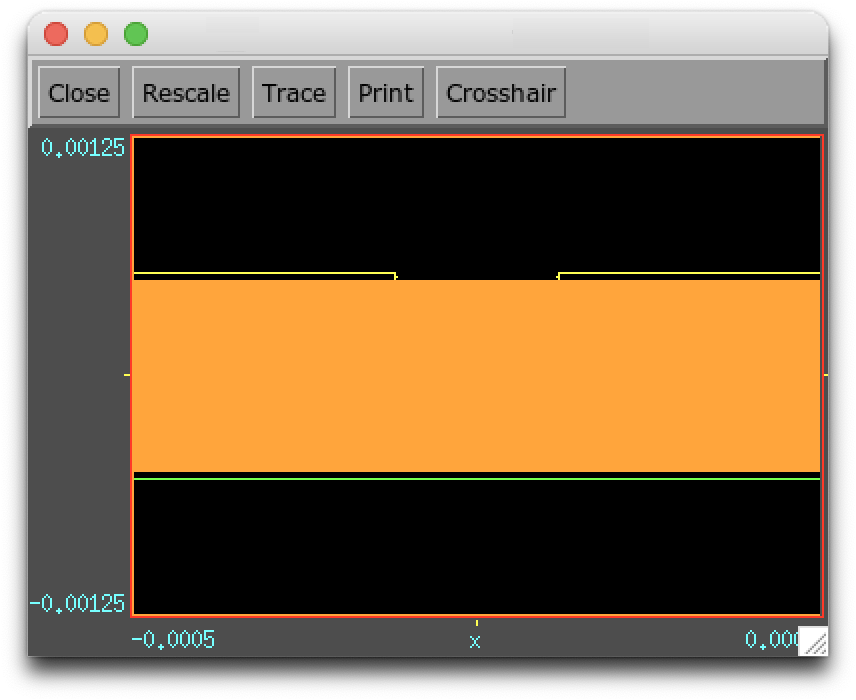
\includegraphics[width=0.9\linewidth]{chapter_4/figures/SRR_no_gap_start.png}
        \caption{}
        \label{fig:SRR_no_gap_start}
    \end{subfigure}%
    \begin{subfigure}{.5\textwidth}
        \centering
        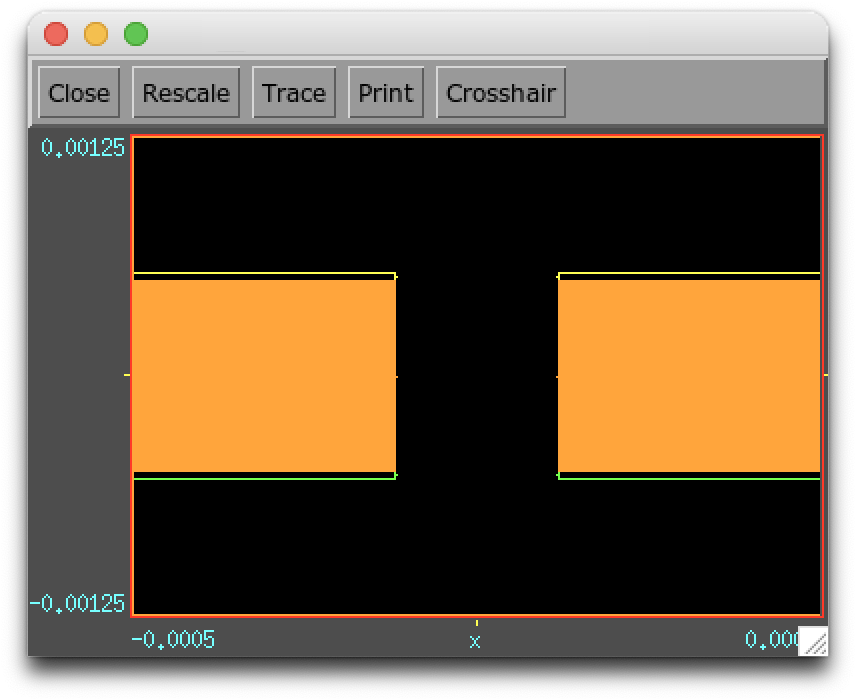
\includegraphics[width=0.9\linewidth]{chapter_4/figures/SRR_with_gap_start.png}
        \caption{}
        \label{fig:SRR_with_gap_start}
    \end{subfigure}
    \caption{A cross section comparison of SRR simulation domain without a hole (a) and with hole (b) in gap.}
    \label{fig:SRR_hole_comparison_start}
\end{figure}

The results of the simulation after it stabilised can be seen in figure \ref{fig:SRR_hole_comparison_stabilise}. The immediate difference that can be observed is the fact that the ions and electrons, represented as blue and orange dots respectively, tended to `sit' deeper into the gap in the case with the through hole. Intuitively, this would make sense as these particles are not colliding with the substrate (which in XOOPIC meant that they were removed from the simulation domain). Additionally, it was hypothesised that strength of the electric field between the top electrodes and the ground plane could potentially play an effect in how deep the ions and electrons penetrate in the gap of the SRR and control the average electron energy.

\begin{figure*}
    \centering
    \begin{subfigure}[b]{0.475\textwidth}
        \centering
        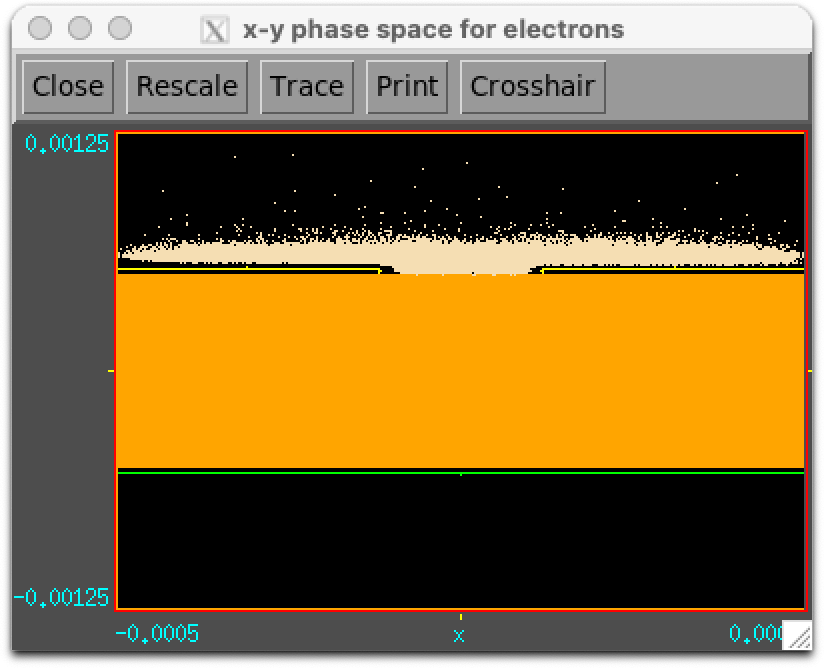
\includegraphics[width=\textwidth]{chapter_4/figures/SRR_no_hole_electrons.png}
        \caption{}
        \label{fig:SRR_no_hole_electrons}
    \end{subfigure}
    \hfill
    \begin{subfigure}[b]{0.475\textwidth}  
        \centering 
        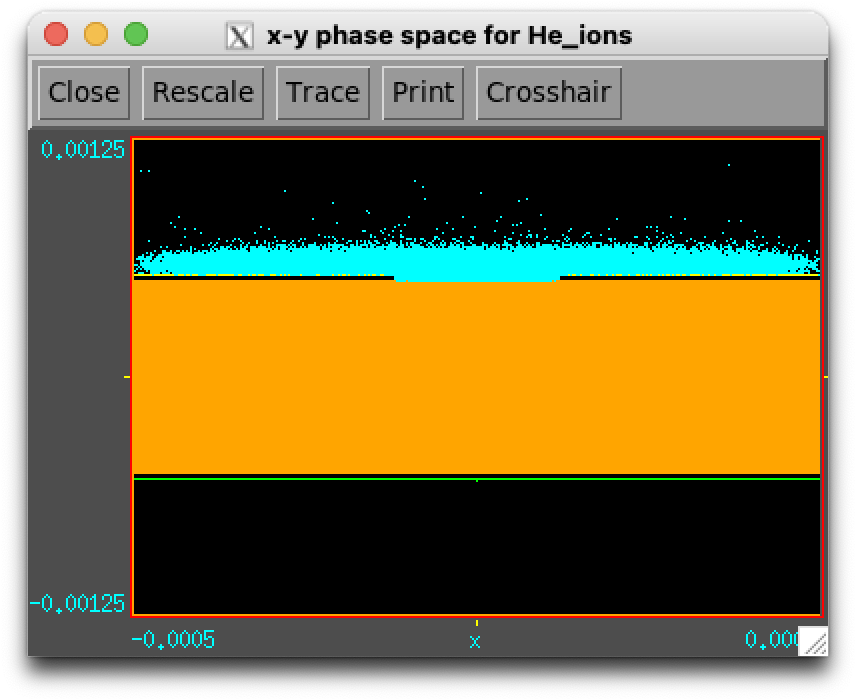
\includegraphics[width=\textwidth]{chapter_4/figures/SRR_no_hole_ions.png}
        \caption{}
        \label{fig:SRR_no_hole_ions}
    \end{subfigure}
    \vskip\baselineskip
    \begin{subfigure}[b]{0.475\textwidth}   
        \centering 
        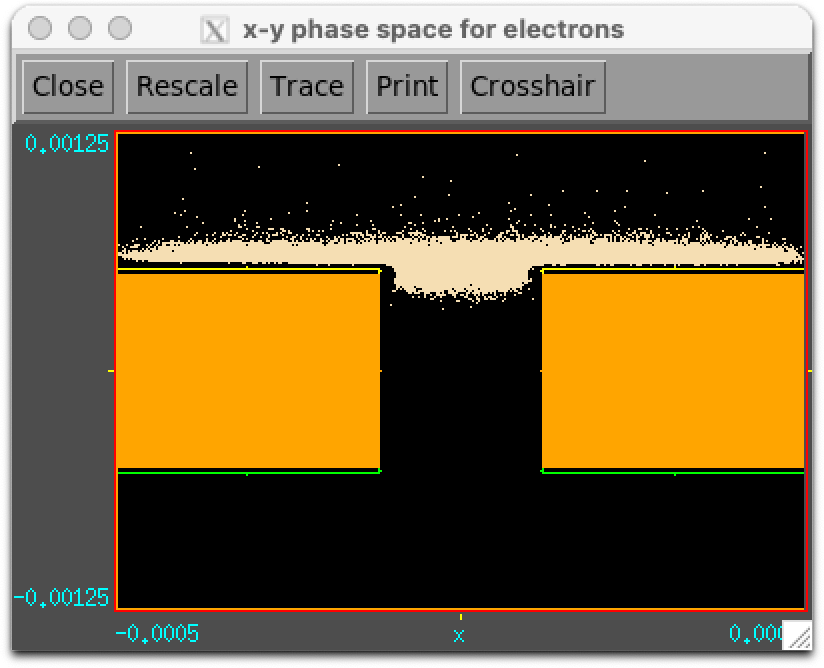
\includegraphics[width=\textwidth]{chapter_4/figures/SRR_with_hole_electrons.png}
        \caption{}
        \label{fig:SRR_with_hole_electrons}
    \end{subfigure}
    \hfill
    \begin{subfigure}[b]{0.475\textwidth}   
        \centering 
        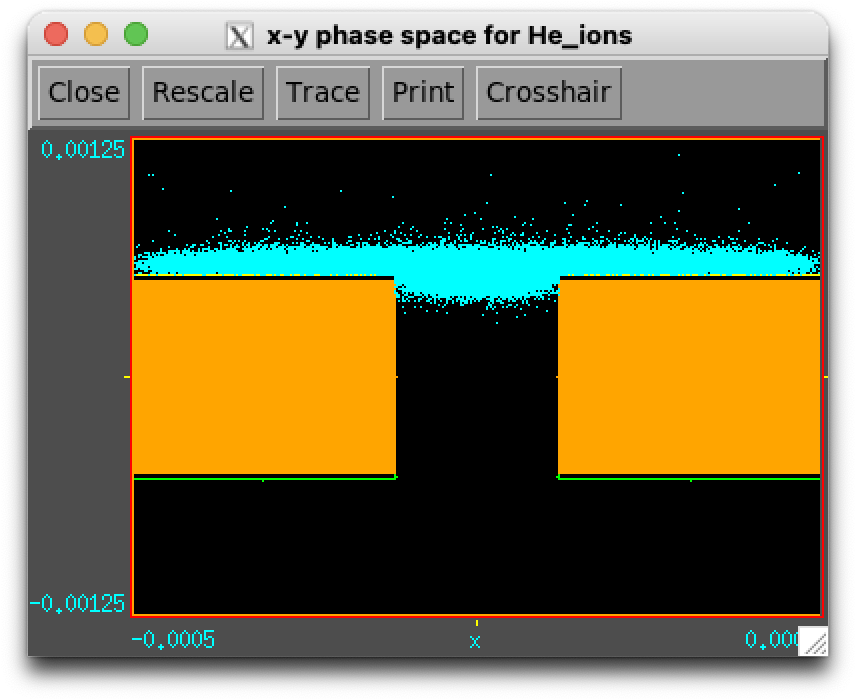
\includegraphics[width=\textwidth]{chapter_4/figures/SRR_with_hole_ions.png}
        \caption{}
        \label{fig:SRR_with_hole_ions}
    \end{subfigure}
    \caption[]
    {\small A comparison of the distribution of electron (a, c) and ions (b, d) in the discharge of the SRR. The top two subfigures (a, b) show the distribution in an SRR with no hole, while the bottom two (c, d) show the distribution in an SRR with a hole in the gap. 
    
    Comparison of SRR with and without hole in gap.} 
    \label{fig:SRR_hole_comparison_stabilise}
\end{figure*}

This leads into the second group of simulations that were run, where the separation distance between the top and bottom electrodes were investigated, which also had the added benefit of identifying  the ideal dielectric substrate thickness to be used when manufacturing the SRR. The parameters used for the size of the gap, the dielectric constant of the substrate, and the potential difference were kept the same as the first group. As for the dielectric thickness, simulations were run with values of 0.2 mm, 0.5 mm, 1.0 mm, 1.5 mm, and 2.0 mm. 

From the cross sectional view of the density plot of electrons in figure \ref{fig:SRR_dielectric_comparison_stabilise}, all simulations performed quite similarly. The electrons seem to extend through the gap by roughly the same distance. However, even though the dielectric thickness did not play a large role in the plasma, it would be preferable to choose a thicker dielectric for the sturdiness of the board. 

The final group of simulations run were to establish the effect of the discharge gap widths. The sizes used were a gap width of 120 $\mu$m, 240 $\mu$m, 360 $\mu$m, and 480 $\mu$m. 

\begin{figure}[h!]
	\centering
	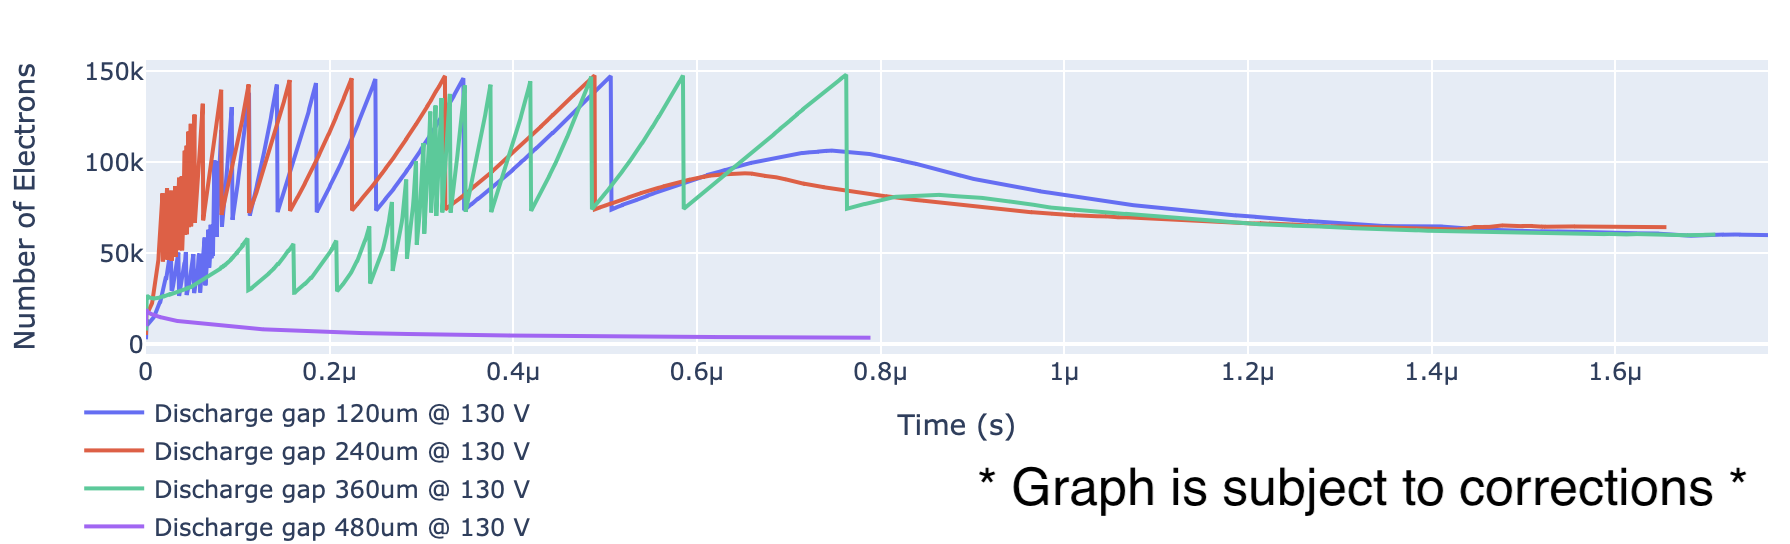
\includegraphics[width=\linewidth]{chapter_4/figures/num_elec_gap.png}
	\caption{Time series plot of number of electrons across different discharge gaps.}
	\label{fig:num_elec_gap}
\end{figure}

The results of these simulations can be seen in figure \ref{fig:num_elec_gap}. From these tests, only three simulations were successful as the run with a gap width of 480 $\mu$m lost all the electrons. The reasons for this behaviour was that the voltage used (150 V) was not sufficient to ignite a discharge, as the electric field in the gap reduces with an increase in gap width. As for the other three runs, the big difference seemed to be the initial growth rate. A gap width of 240 $\mu$m appeared to be the optimum. One would expect that the smallest gap width would perform the best, however as seen by Paschen's law (refer to Chapter \ref{sec:paschens_law}), reducing the distance between electrodes too much would cause the electrons to be simply lost to the electrode. This could possibly explain why the run with a 120 $\mu$m gap performed worse than the run with a gap width of 240 $\mu$m.

\begin{figure*}
    \centering
    \begin{subfigure}[b]{0.475\textwidth}
        \centering
        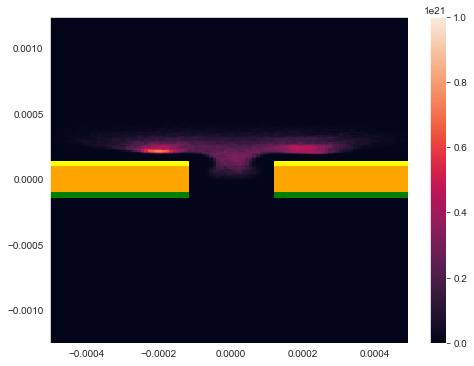
\includegraphics[width=\textwidth]{chapter_4/figures/SRR_dielectric_1.png}
        \caption{}  
        \label{fig:SRR_dielectric_0.2mm}
    \end{subfigure}
    \hfill
    \begin{subfigure}[b]{0.475\textwidth}  
        \centering 
        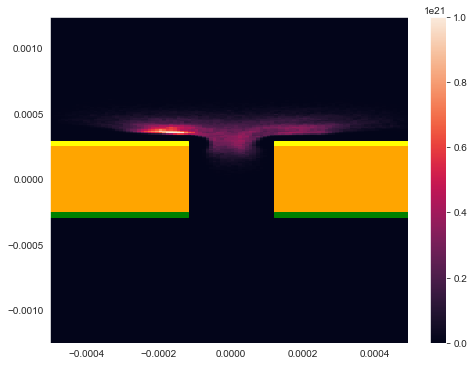
\includegraphics[width=\textwidth]{chapter_4/figures/SRR_dielectric_2.png}
        \caption{}   
        \label{fig:SRR_dielectric_0.5mm}
    \end{subfigure}
    \vskip\baselineskip
    \begin{subfigure}[b]{0.475\textwidth}   
        \centering 
        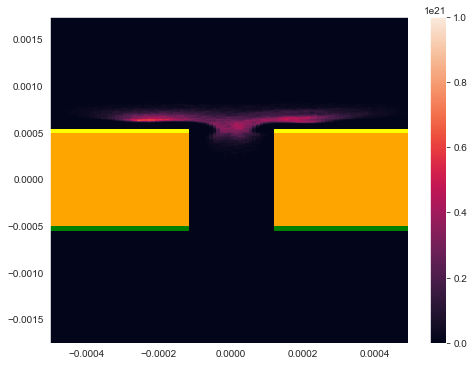
\includegraphics[width=\textwidth]{chapter_4/figures/SRR_dielectric_3.png}
        \caption{}    
        \label{fig:SRR_dielectric_1.0mm}
    \end{subfigure}
    \hfill
    \begin{subfigure}[b]{0.475\textwidth}   
        \centering 
        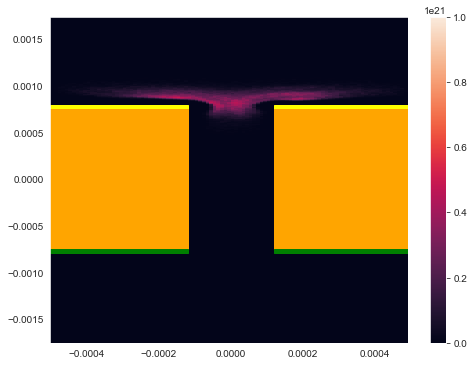
\includegraphics[width=\textwidth]{chapter_4/figures/SRR_dielectric_4.png}
        \caption{}   
        \label{fig:SRR_dielectric_1.5mm}
    \end{subfigure}
    \vskip\baselineskip
    \begin{subfigure}[b]{0.475\textwidth}   
        \centering 
        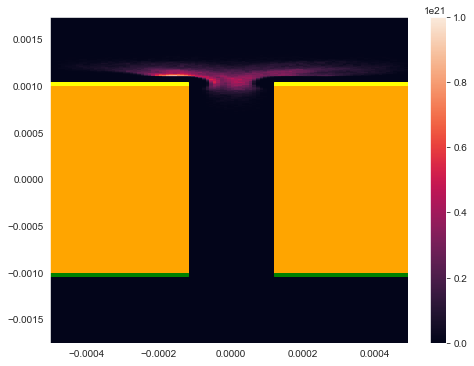
\includegraphics[width=\textwidth]{chapter_4/figures/SRR_dielectric_5.png}
        \caption{}    
        \label{fig:SRR_dielectric_2.0mm}
    \end{subfigure}
    \caption[]
    {\small Comparison of dielectric thickness of 0.2 mm (a), 0.5 mm (b), 1.0 mm (c), 1.5 mm (d), and 2.0 mm (e) on the SRR.} 
    \label{fig:SRR_dielectric_comparison_stabilise}
\end{figure*}

\subsection{Design}

Armed with this information, a design of the SRR to be used was made. The first step was to select the PCB substrate to be used, as its dielectric constant is a central parameter for all other calculations of the SRR. The material selected was the RO4350B\textsuperscript{TM} material from Rogers corporation. This specific material was chosen as it is designed for high power UHF designs, and its relatively low fabrication costs. Additionally, the RO4350B\textsuperscript{TM} material did not require any special treatments or procedures to introduce a through hole. According to its data sheet, the RO4350B\textsuperscript{TM} board has a dielectric constant of 3.66, and a dissipation factor of 0.0031 (which can be converted to the quality factor). In the data sheet, these values were tested at a frequency of 2.5 GHz. However, an assumption was made during the design process that these values would be approximately equivalent for the operational frequency selected.  

Choosing the resonant frequency for the SRR required striking a compromise. Ideally, a higher resonant frequency would improve the quality factor, reducing power losses and making it more likely that a plasma discharge occurs. However, a frequency that is too high would increase power requirements required to drive the SRR. An additional drawback to using higher frequencies is that as seen in equation \ref{eq:resonant_frequency}, increasing the frequency causes a decrease in the wavelength, which in turn reduces the size of the SRR. While this is not directly a problem, a smaller ring for the SSR would require significantly tighter manufacturing tolerances which in turn drive up the cost of production. Therefore, a target frequency of 500 MHz was chosen to strike a balance between the these factors. 

Feeding this number into equation \ref{eq:resonant_frequency}, the corresponding wavelength was 0.314 m. Since the circumference of the SRR is given as $\lambda/2$, this meant that the design had a circumference of 15.71 cm; which gives the SRR a radius of approximately 2.5 cm. 

The next step was to determine the characteristic impedance. Conventionally, this impedance should be close to the value of the input impedance, which for power supply used was 50 $\Omega$. As mentioned earlier in this chapter, three factors dictate the value of this parameter. The dielectric constant of the substrate was 3.66, a fixed value based on the material used. As stated in the previous section, a thicker dielectric substate would be preferable. The RO4350B\textsuperscript{TM} material came in a thickness of 0.5 mm, 0.8 mm, and 1.55 mm; with the costs increasing with thickness. Thus, as a compromise between the structural rigidity PCB and cost, a thickness of 0.8 mm was selected. By using the equations \ref{eq:wheeler_microstrip}-\ref{eq:wheeler_effective_w}, a trace width of approximately 1.7 mm would produce a characteristic impedance of 50.1 $\Omega$.

Finally using equation \ref{eq:offset_angle}, the offset angle of the SRR was calculated. As from the datasheet, the dissipation factor of the RO4350B\textsuperscript{TM} material is 0.0031. The reciprocal of this value was taken to determine the quality factor, which was 323. This would give a gap with an offset angle of 7.99. Again based on the simulations above, the ideal gap width was 240 $\mu$m, however the minimum size drill hole size would be the limiting factor when manufacturing the device, hence the gap width was slightly increased to 250 $\mu$m.

With these parameters known, the next stage was to create the PCB design. This was done using the open-sourced PCB design software called \textit{KiCad}\footnote{https://www.kicad.org}. One benefit of using KiCad was the output files were natively supported by  the PCB manufacturer used, \textit{EuroCircuits}\footnote{https://www.eurocircuits.com}. 

An illustration of the final design can be seen in figure \ref{fig:SRR_cad}. As seen from the figure, four SRR designs were made. These were done to test various gap designs that could not be replicated using XOOPIC simulations. These designs could be broken down into two categories: single versus multiple drill hole in the SRR gap; and the presence versus absence of `finger-like' copper pours next to the SRR gap. The permutations of these categories resulted in the four designs, with a close up image of each shown in figure \ref{fig:SRR_cad_close_up}. All four designs used an SMA connector as the input source. 

\pagebreak

\begin{figure}[h!]
	\centering
	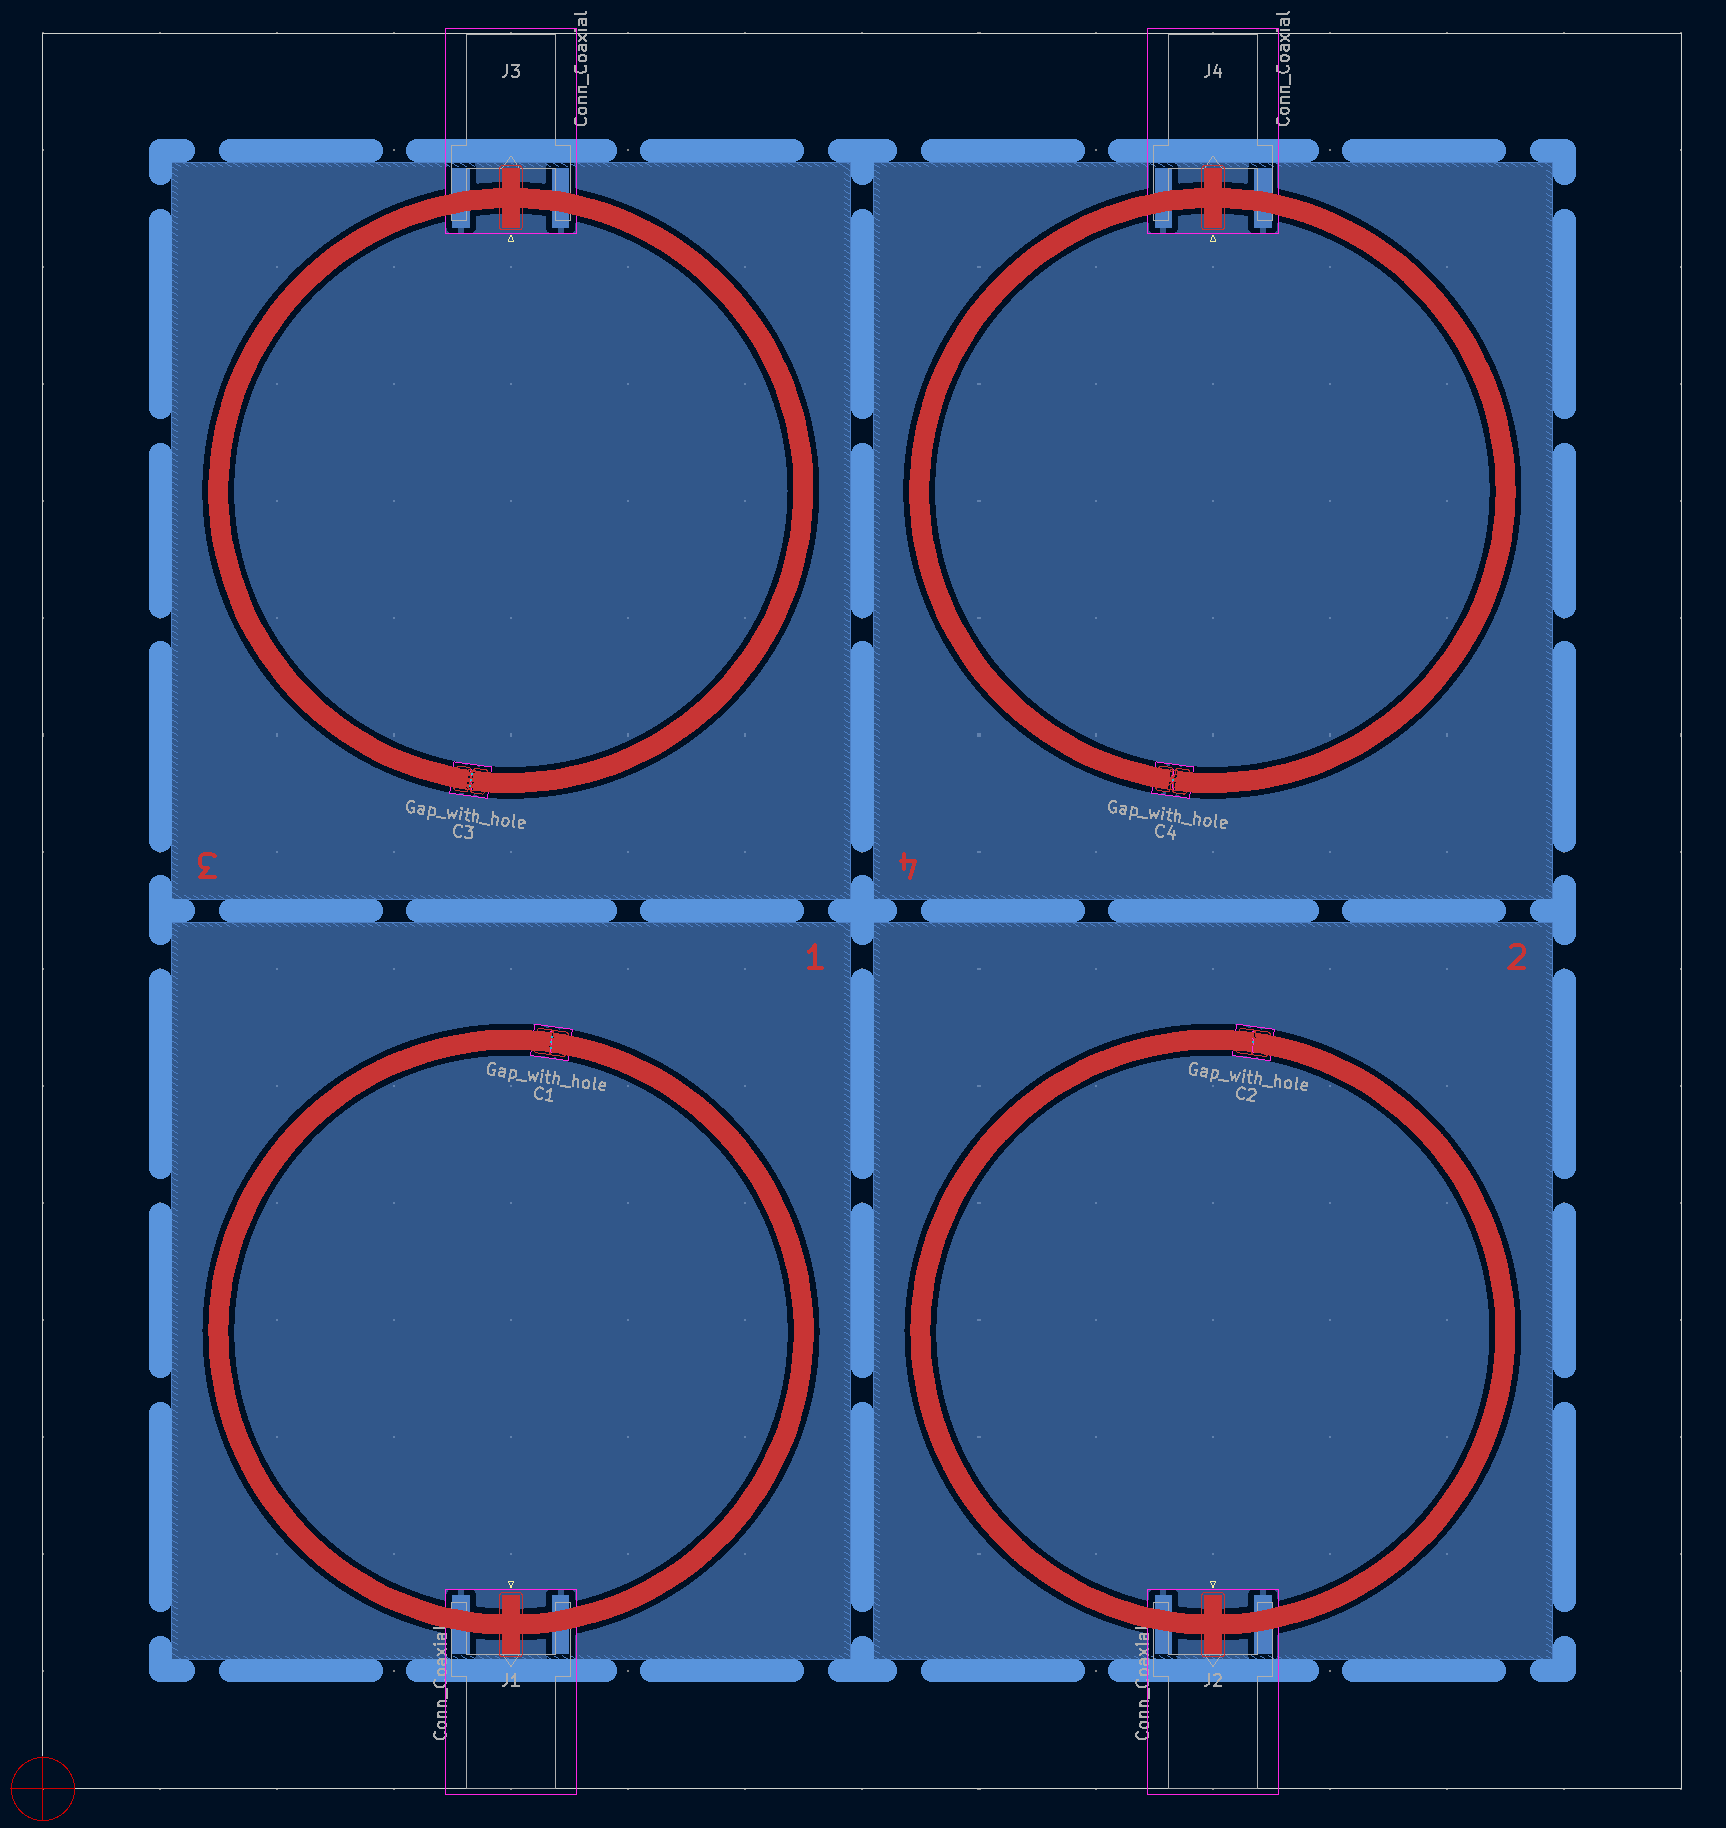
\includegraphics[width=\linewidth]{chapter_4/figures/SRR_CAD.png}
	\caption{PCB schematic of SRR panels in the KiCad software suite.}
	\label{fig:SRR_cad}
\end{figure}

\begin{figure}
    \centering
    \begin{subfigure}[b]{0.475\textwidth}
        \centering
        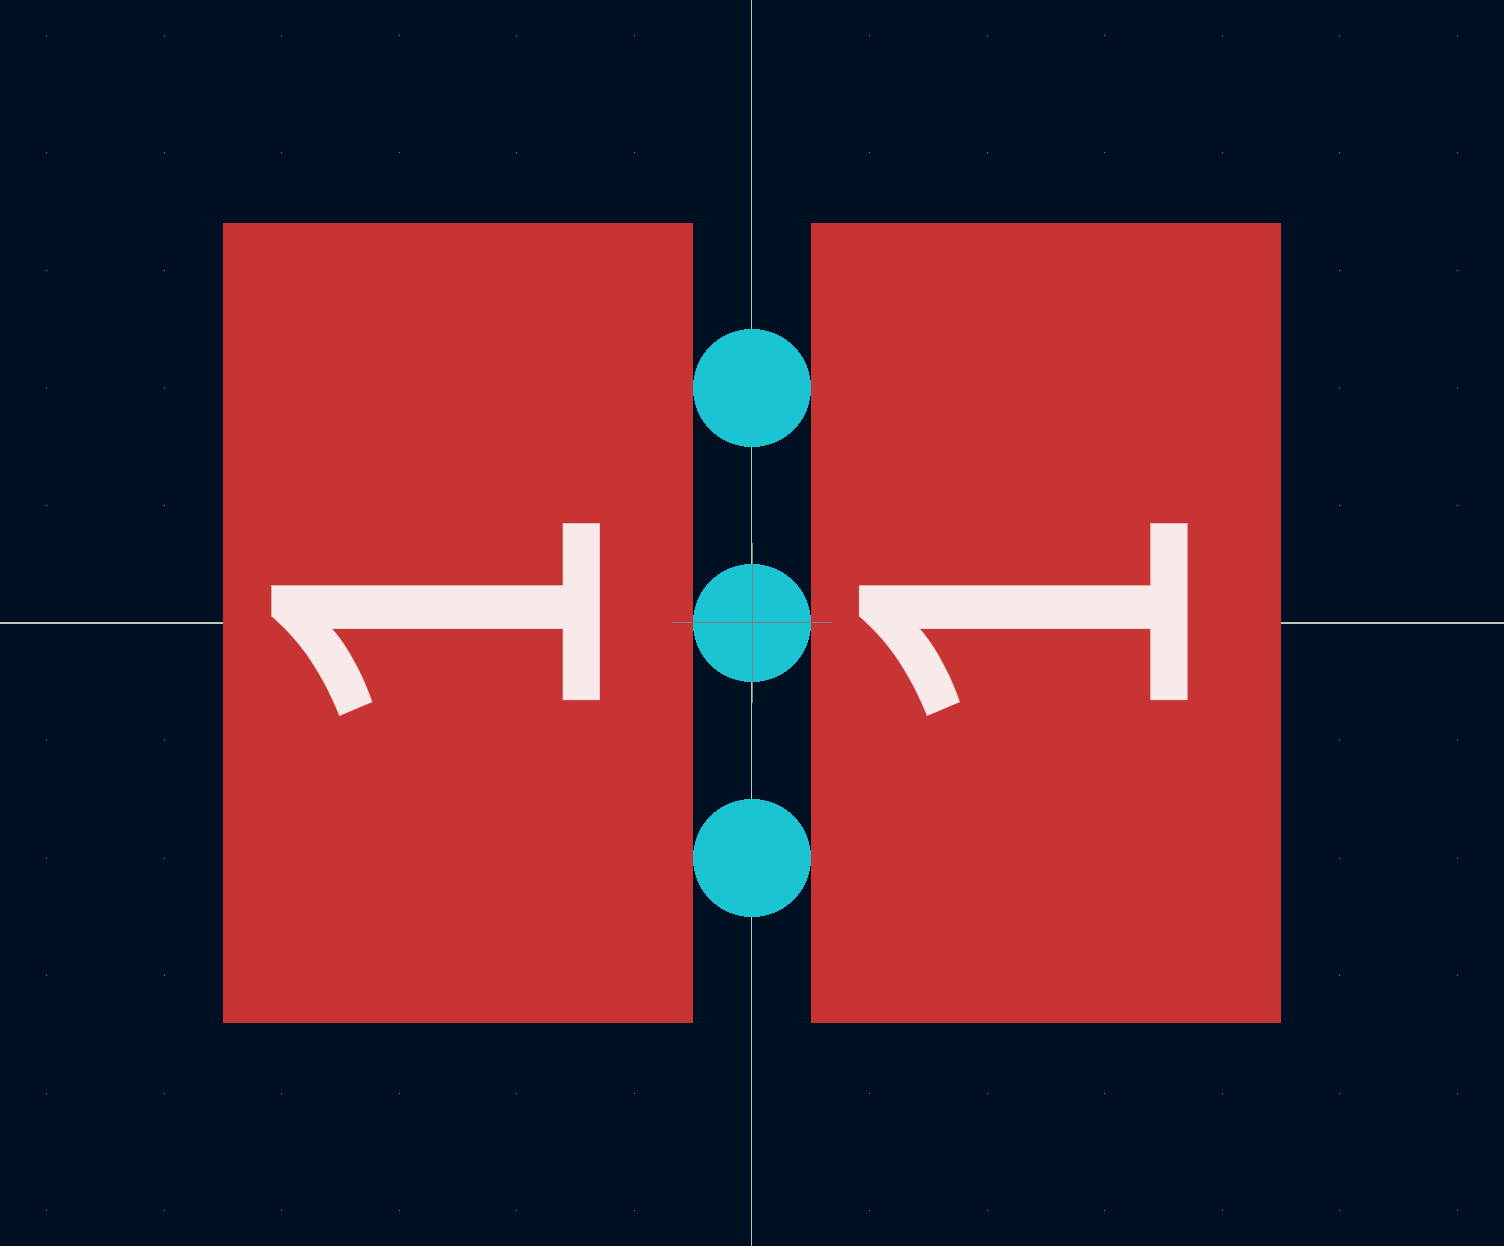
\includegraphics[width=\textwidth]{chapter_4/figures/SRR_CAD_hole_1.png}
        \caption{}
        \label{fig:design_1}
    \end{subfigure}
    \hfill
    \begin{subfigure}[b]{0.475\textwidth}  
        \centering 
        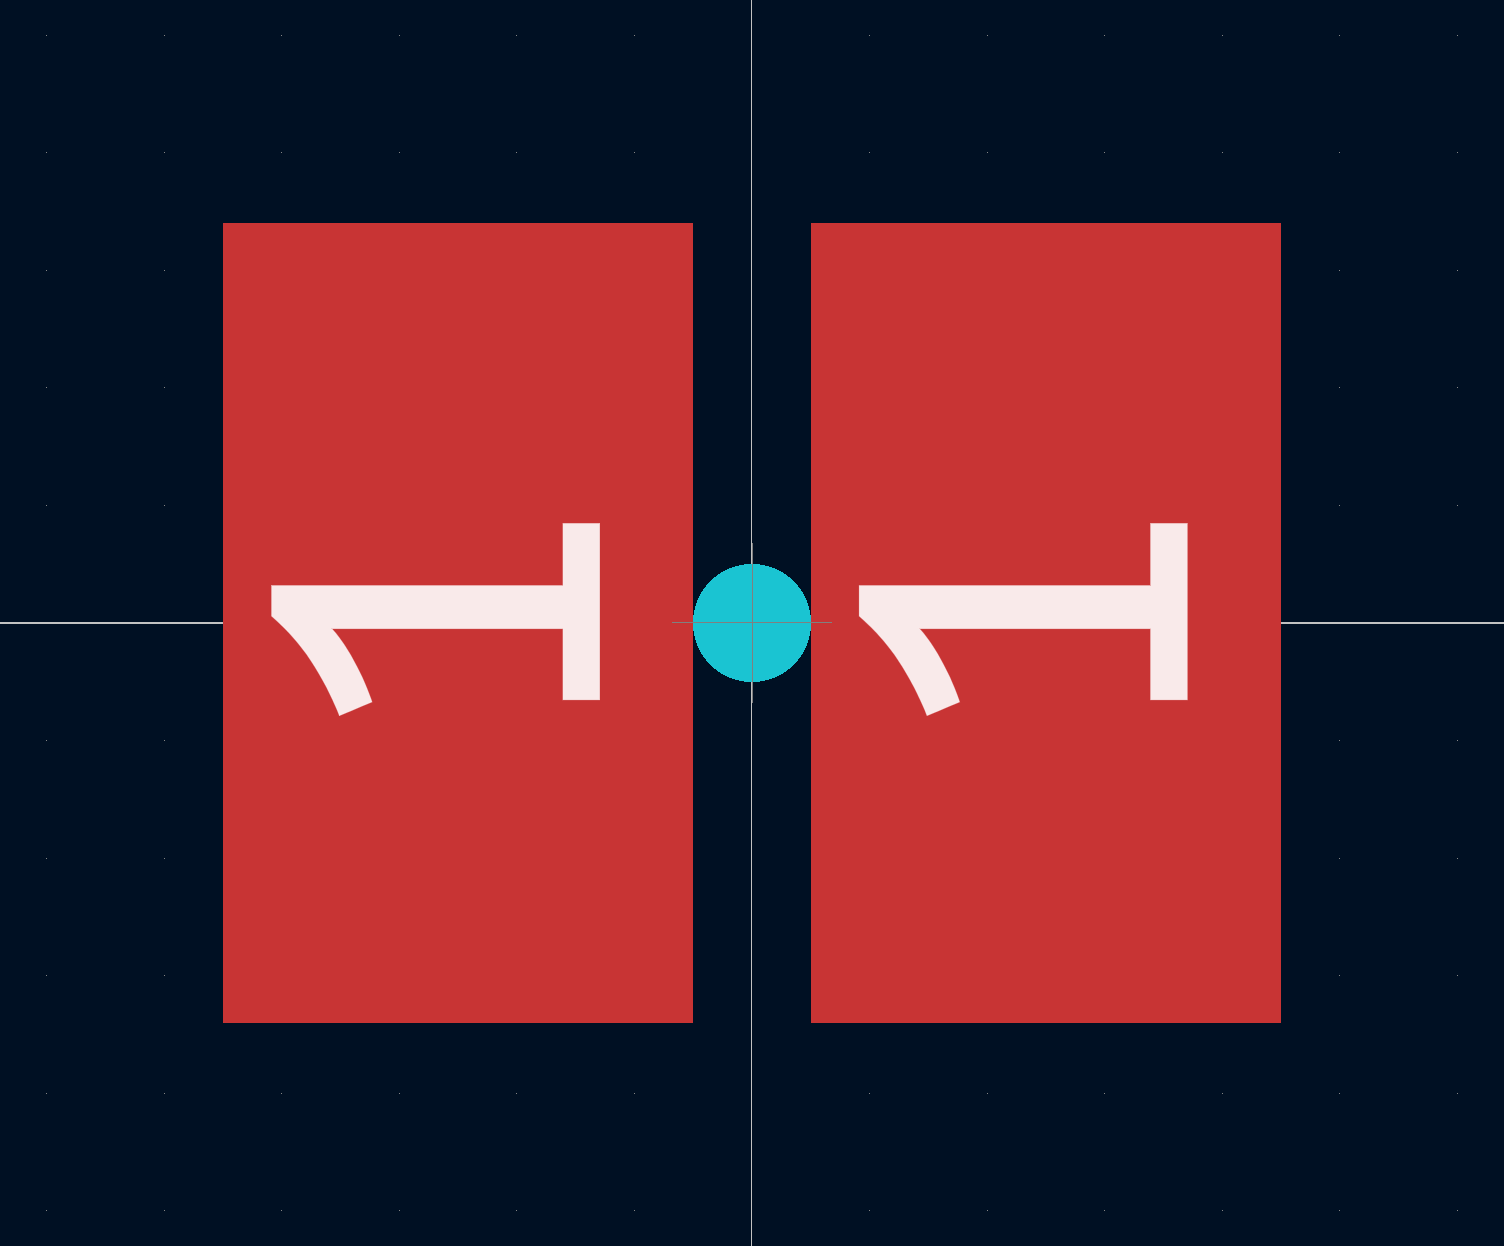
\includegraphics[width=\textwidth]{chapter_4/figures/SRR_CAD_hole_2.png}
        \caption{}
        \label{fig:design_2}
    \end{subfigure}
    \vskip\baselineskip
    \begin{subfigure}[b]{0.475\textwidth}   
        \centering 
        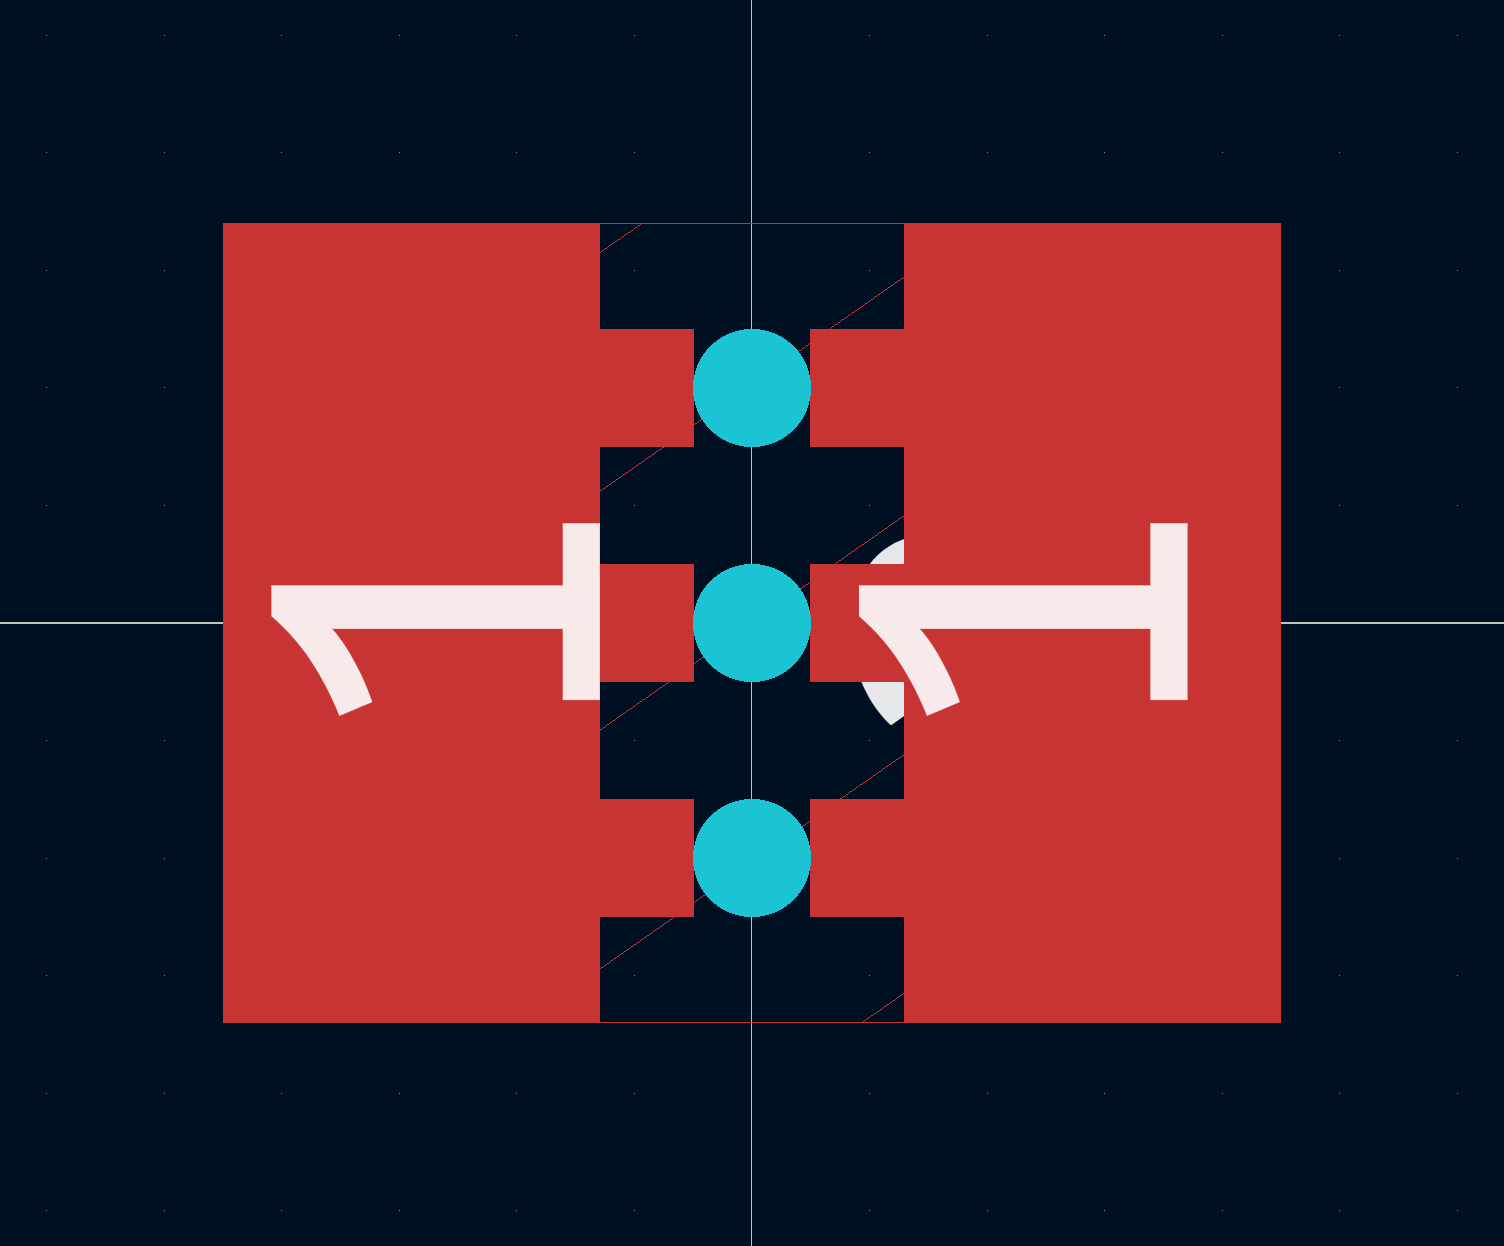
\includegraphics[width=\textwidth]{chapter_4/figures/SRR_CAD_hole_3.png}
        \caption{}
        \label{fig:design_3}
    \end{subfigure}
    \hfill
    \begin{subfigure}[b]{0.475\textwidth}   
        \centering 
        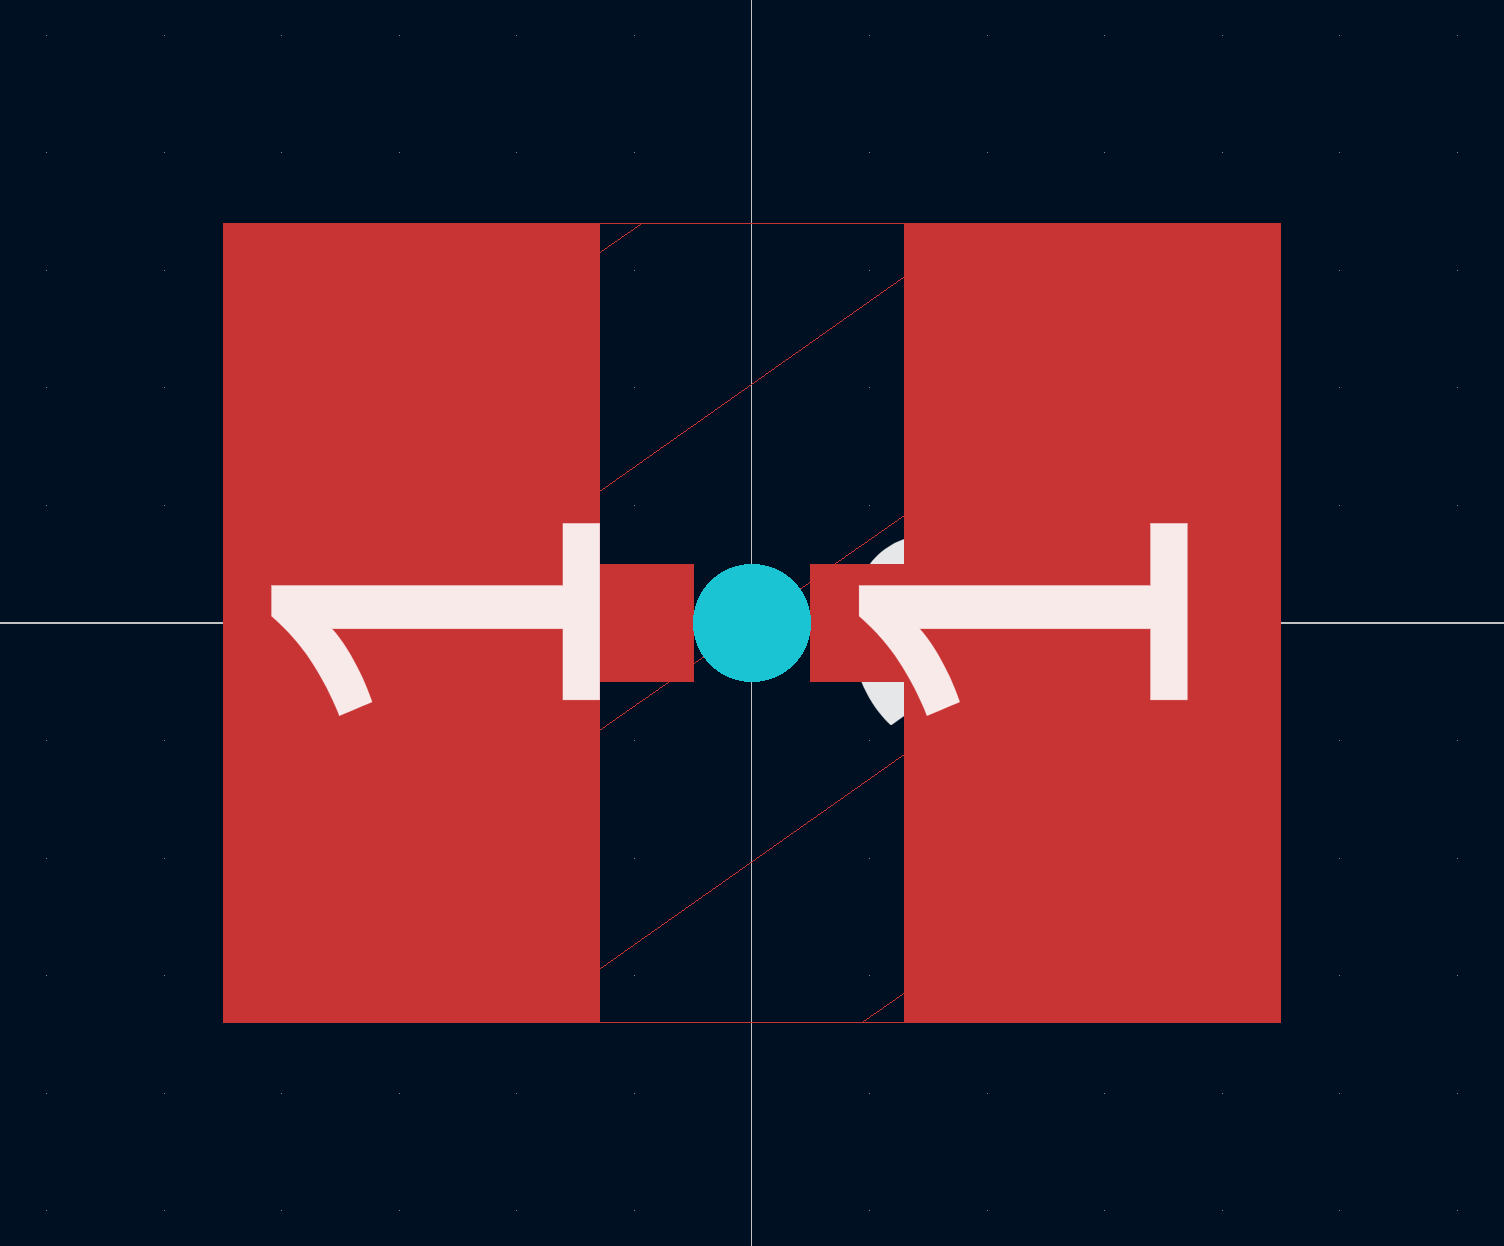
\includegraphics[width=\textwidth]{chapter_4/figures/SRR_CAD_hole_4.png}
        \caption{}
        \label{fig:design_4}
    \end{subfigure}
    \caption{\small SRR gap designs with multiple holes (a, c) versus single holes (b, d). The designs in the lower two subfigures (c, d) have the presence of `finger-like' copper pours next to the holes.} 
    \label{fig:SRR_cad_close_up}
\end{figure}





%%\pagebreak
\section{Testing}
\subsection{Scattering Parameters}

Once the PCBs were manufactured, and the SMA connectors soldered on to the SRR panel, a comparison between the theoretical calculations of the SRR and its real world characteristics could be made. This was achieved best evaluating its \textit{scattering parameters} (S-parameters) using a vector network analyser (VNA). 

In essence, the S-parameters are a measurement of the transmitted and reflected power of a device under test, in this case the SRR, as a function of frequency. The output of this test is a description of the device in terms of amplitude and phase across a given sweep of frequencies. Since the SRR only had a single port, it only had one S-parameter, referred to as the S$_{11}$ or the reflection coefficient. This is a ratio of the output voltage of the port to the input voltage going into the device. 

For the test, the VNA was first calibrated then a sweep was performed between the frequencies of 100 MHz to 1 GHz. Since the SRR was designed to resonate at approximately 500 MHz, this should place a single largest peak at roughly the centre of the frequency range, and the broad range would also capture any shifts in the resonant frequency due to manufacturing tolerances. 

\begin{figure}[h!]
	\centering
	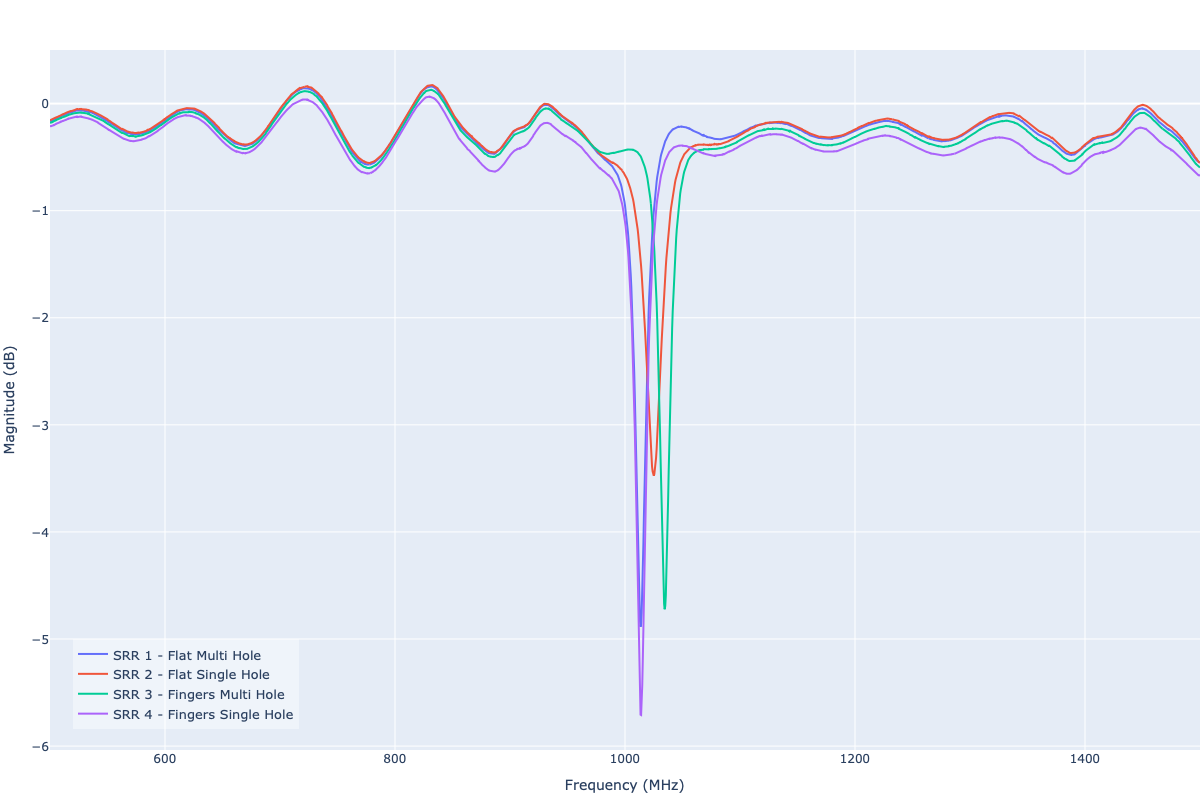
\includegraphics[width=\linewidth]{chapter_4/figures/S11.png}
	\caption{Reflection coefficient (S$_{11}$) of SRR in dB.}
	\label{fig:SRR_s11}
\end{figure}


Figure \ref{fig:SRR_s11} shows the data from the S$_{11}$ test, with the y-axis indicating the magnitude of attenuation (in decibels) at a given frequency. Readers will immediately notice the fact that there are two peaks in the SRR, not just one. The peaks have a central frequency of 554 MHz and 753 MHz respectively. The first of these peaks would be inline with the margin of error for the designed resonant frequency. The second peak on the other hand, represents some additional resonance in the SRR circuit. This could be introduced by a number of factors, such SMA connector itself or the presence of gaps on the underside along the ground ring. While this second peak indicates a stronger resonance, as seen by the larger attenuation and higher quality factor, it is not possible to ignite a plasma at that frequency. This is because, as stated earlier in this chapter, the formation of the plasma is governed by the relationship between the wavelength of the input power and the circumference of the SRR.

As for first peak at 554 MHz, it appeared to have a much lower quality factor in the real world. This implies that the assumption made in the design phase regarding the dielectric constant and dissipation factor were incorrect. While this does not necessarily affect the plasma discharge, it does mean that a higher power is going to be required to ignite the plasma.

\subsection{Experimental Setup}

Once the true resonant frequency was determined, the next step was to setup the experiment. Note that this is not the final setup to be used for recirculating the gases, instead it was used to reliably ignite a plasma from the SRR in order to characterise it and understand its behaviour. An illustration of the setup is seen in figure \ref{fig:SRR_setup}.

\begin{figure}[h!]
	\centering
	\includegraphics[width=\linewidth]{chapter_4/figures/SRR_setup.png}
	\caption{Schematic of experimental setup.}
	\label{fig:SRR_setup}
\end{figure}

In the setup, there are two mass flow controllers by MKS Instruments. For the time being, these are only controlling the flow of helium gas into the setup; the introduction of carbon dioxide gas is discussed in the next chapter. The first one (MFC$_1$)  is positioned on the bottom side of the SRR, whilst the second one (MFC$_2$) controls the flow to the chamber. The reason for two separate mass flow controllers is that the size of the aperture of the SRR is quite small (with a diameter of 0.25 mm), hence only using one controller to pressurise the entire apparatus at 760 Torr (which is one atmosphere) would take a long time. Thus, MFC$_2$ is used to maintain pressure the pressure of the chamber whilst MFC$_1$ maintains a flow of Helium through the gap of the SRR. 

The SRR device is oriented so that the Helium flows from the bottom (i.e. the ground ring) to top; (i.e. the AC ring). This is because the plasma discharge occurs at the top of the ring, thus when used later in the epoxidation process, this is the side that is going to face the liquid co-reactant. A photograps of the plasma can be seen in figure \ref{fig:SRR_plasma}. 

\begin{figure}[h!]
	\centering
	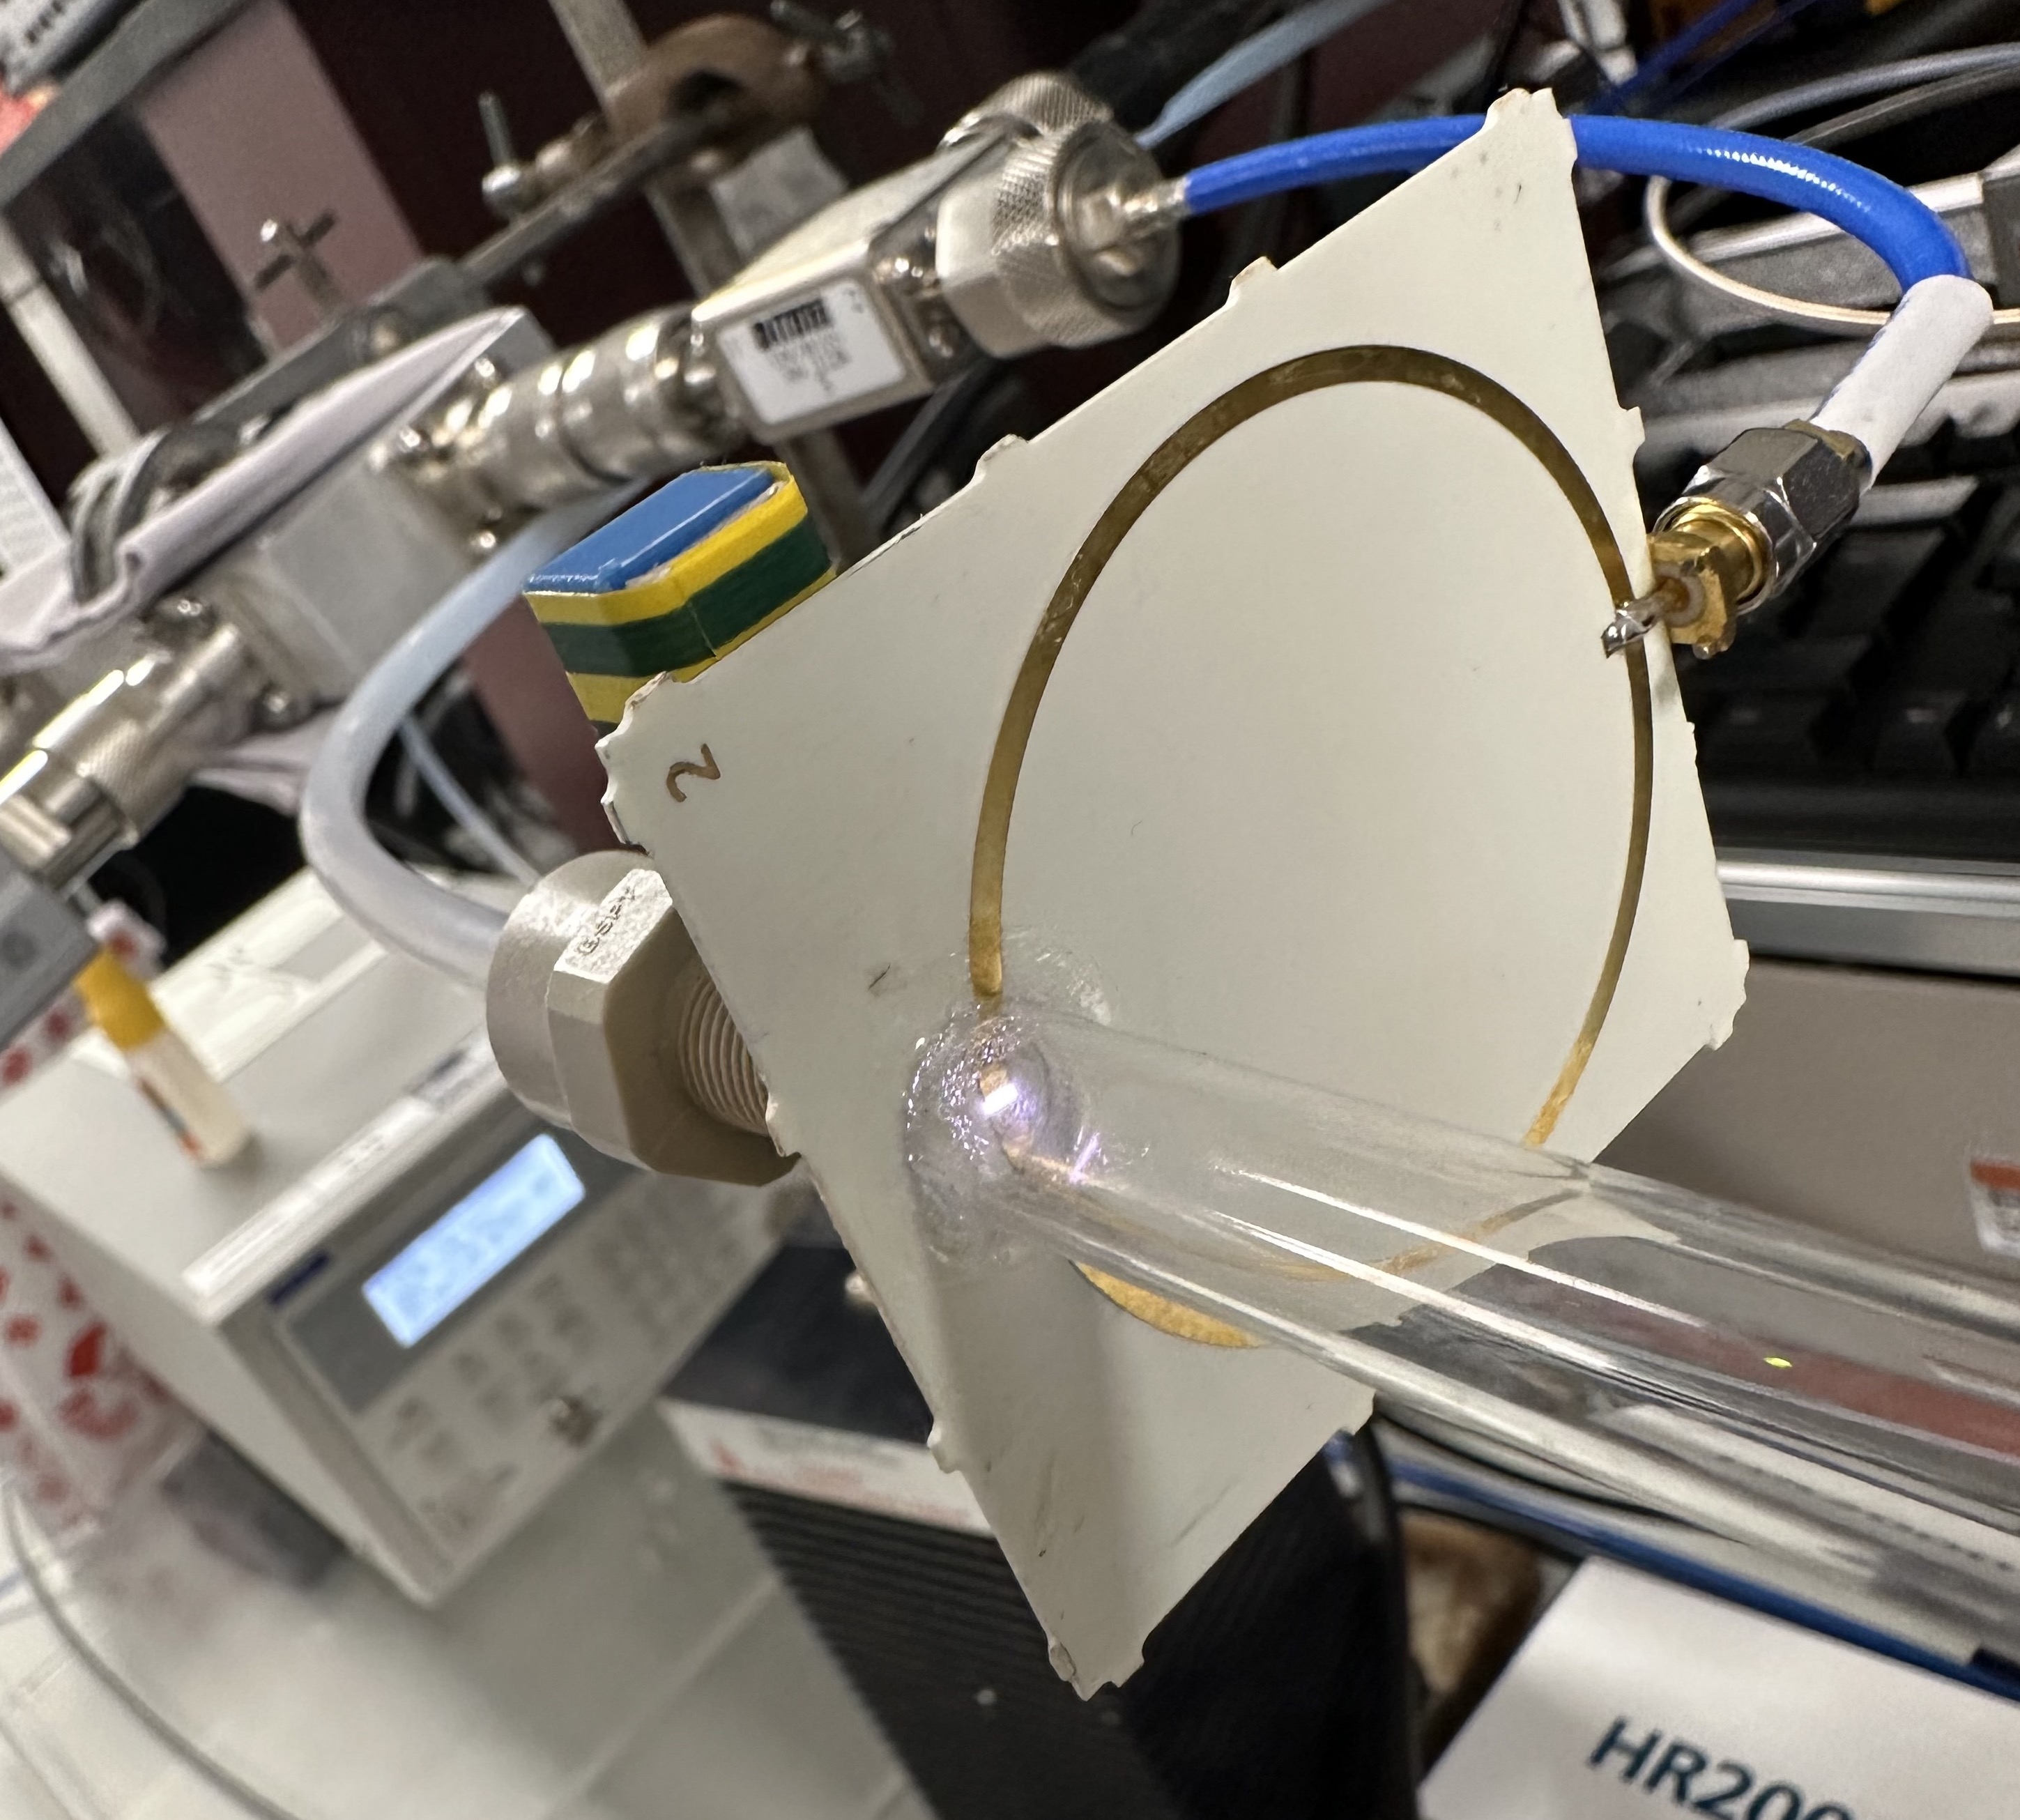
\includegraphics[width=0.55\linewidth]{chapter_4/figures/plasma.jpeg}
	\caption{Photograph of plasma discharge in the gap of the SRR.}
	\label{fig:SRR_plasma}
\end{figure}


In terms of the electronics, the the SRR is powered by a signal generator (Aim-TTi TGR2050), capable of generating frequencies up to 2 GHz, and a linear amplifier (Amplifier Research 50W1000A), with a maximum power output of 50 W. This is connected to a bi-directional coupler (Mini-Circuits ZGBDC20-33H-S+) to allow for the accurate measurement of the forward path and the reverse path of the microwave signals from the power supply and SRR respectively. These signals are monitored using a pair of USB power meters (Mini-Circuits PWR-SEN-4GHz, Mini-Circuits PWR-SEN-6LRMS-RC). One note regarding the power meters, the first power meter (PM$_1$) has a maximum power input of 100 mW, whilst the second one (PM$_2$) has a maximum reading of 10 mW. This is because, when the SRR is at resonance, only a small amount of signal is reflected back. 

\subsection{Plasma performance}

Now that the SRR was connected to the setup, there may be a slight change in the resonant frequency due to coupling with the rest of the electronics. However, with the use of the bi-directional couplers and the power meters, it is possible to find the frequency of resonance of the overall setup. This is achieved by keeping the input power of the power supply fixed, but varying its frequency. This way, the reading of the forward wave would be constant, with the power of the reflected wave changing. 

For this, the input power was kept at a constant 10 mW. This was chosen as it was a low enough power to not ignite a plasma (which in turn would change the resonance characteristics of the SRR). As for the frequencies, a sweep was performed between 500 MHz to 600 MHz. The results of this can be seen in figure \ref{fig:reflected_power_SRR.png}. 

\begin{figure}[h!]
	\centering
	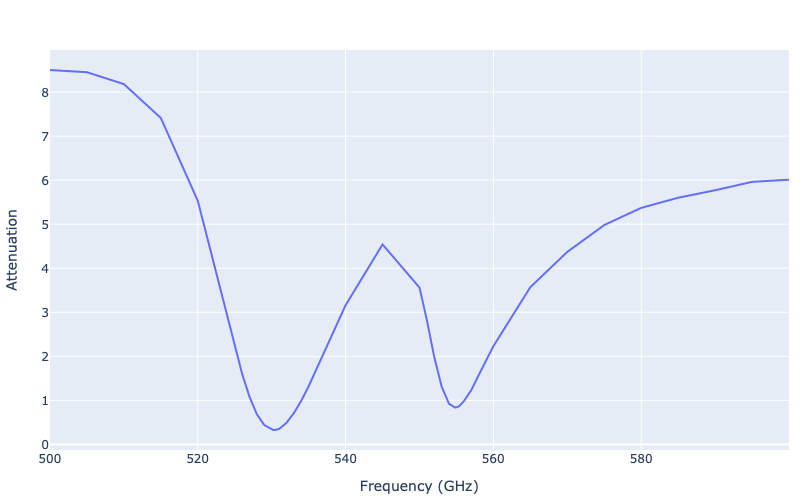
\includegraphics[width=\linewidth]{chapter_4/figures/reflected_power_SRR.png}
	\caption{Reflection power of SRR when connected to the setup in mW.}
	\label{fig:reflected_power_SRR.png}
\end{figure}

Two dips can be seen in the data. These dips correspond to the frequencies that cause an attenuation in the SRR. As expected, a drop in return power can be seen at 554 MHz (more precisely, it is 554.8 MHz), which is inline with the S-parameters measurements. However, a second dip is seen at 530 MHz (530.4 MHz specifically). Notably, this drop of return power at 530 MHz is lower than that of the drop at 554 MHz; with the readings being 0.33 mW and 0.84 mW respectively. As such, it can be concluded that 530.4 MHz is resonant frequency of the SRR connected to the rest of the setup. This conclusion is backed up by the fact that the plasma only ignites at that frequency, and not at 554 MHz.

Once ignition was achieved, the next steps were to evaluate the performance of the plasma. The first thing to evaluate was the ignition power of the SRR. This is because, igniting plasma at higher pressures tends to be slightly more inefficient compared to lower pressures. Thus, the ignition power was tested at various pressures to determine the minimum power required to get a plasma to from with the SRR. 

To obtain this data, first the pressure of the chamber was fixed. Then input power to the SRR was increased gradually until the self-ignition of the plasma. The power value was noted, and the input power was reduced back to the minimum value and the process was repeated. In total, there were five power readings taken at each pressure to account for outliers. This data is shown in figure \ref{fig:ignition_power}. Each point in the figure denotes the average ignition power at that pressure, with the error bars denoting the standard deviation in the data collected. Do note that x-axis of this graph was plotted in logarithmic scale. 

\begin{figure}[h!]
	\centering
	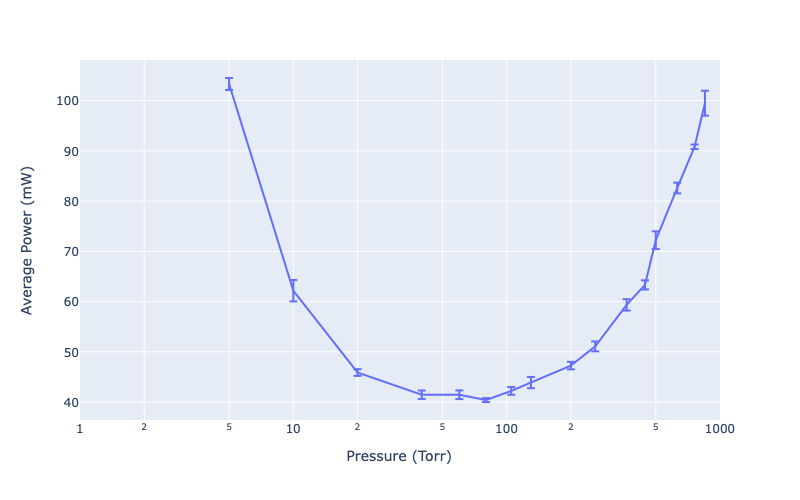
\includegraphics[width=\linewidth]{chapter_4/figures/ignition_power.png}
	\caption{Ignition power of SSR, in mW, across a pressure range of 5 Torr to 850 Torr.}
	\label{fig:ignition_power}
\end{figure}

As seen by the graph, the minimum power required to ignite the plasma was just 40.4 mW. While this is fairly small, it could be better as the real world quality factor of the SRR was lower than anticipated. While this minimum ignition power was achieved at 80 Torr, the power remained relatively low across a broad range of pressures, ranging from 40 Torr to 105 Torr, with the ignition power hovering around 41-42 mW. As the pressure decreased below 40 Torr, the ignition power required increased steeply up to a pressure of 5 Torr where the readings maxed out the range of the power meter. It is also important to note that at 5 Torr, while the plasma self-ignited, it did take significantly longer when compared to the ignition at other pressures. As for pressures above 105 Torr, the ignition power also increased, though at a much slower rate. At 760 Torr, the average power required to ignite the plasma was 90.8 mW. The testing was carried out past 760 to determine the upper bound pressure that a plasma could be ignited with the equipment in the setup; this value was at 850 Torr. 

From the data in figure \ref{fig:ignition_power}, it can be concluded that the most efficient way to ignite a plasma with this SRR would be to first pressurise the chamber to approximately 100 Torr. Then, once the plasma is ignited, the pressure can be increased back to 760 Torr. 





